Modules mentioned above are grouped \modified{according its signature. An \textit{abstract module} is a module that represents all modules with the same signature.} For example, the module showed in Figure~\ref{fig:om} is a \om{} based on an abstract module that receives a configuration and returns a neighborhood. %In that sense, an example of a concrete \om{} (or just \om{}) can be a function receiving a configuration, and returning a neighborhood constituted by $N$ configurations which only differ from the input configuration in one entry.

In this stage an \INTROas{} is coded using \posl{}. It takes abstract modules as {\it parameters} and combines them through operators. Through the \as, we can also decide which information to send to other solvers. % by using some operators to send the result of a computation module (see below). In the following we present a formal and more detailed specification of \posl{}'s operators. 

The \as{} is the solver's backbone. It joins the \oms{} and the \opchs{} coherently. It is independent from the \oms{} and \opchs{} used in the solver. It means that modules can be changed or modified during the execution, respecting the algorithm structure. Each time we combine some of them using \posl's operators, we are creating a \INTROcm. Here we formally define the concept of \textit{module} and \INTROcm.

\begin{definition}
\label{def:module}
Denoted by the letter $\mathcal{M}$, a {\bf module} is:
\begin{enumerate}\renewcommand{\labelitemi}{\scriptsize$\blacksquare$}
\item a \om{}; or
\item a \opch{}; or
\item $\left[\text{OP } \mathcal{M}\right]$, which is the composition of a module $\mathcal{M}$ to be executed sequentially, returning an output depending on the nature of the unary operator \emph{OP}; or\label{subdef:seq_uni}
\item $\left[\mathcal{M}_1 \text{ OP } \mathcal{M}_2\right]$, which is the composition of two modules $\mathcal{M}_1$ and $\mathcal{M}_2$ to be executed sequentially, returning an output depending on the nature of the binary operator \emph{OP}; or\label{subdef:seq}
\item $\lbk\mathcal{M}_1 \text{ OP } \mathcal{M}_2\rbk_p$, which is the composition of two modules $\mathcal{M}_1$ and $\mathcal{M}_2$ to be executed, returning an output depending on the nature of the binary operator \emph{OP}. These two modules will be executed in parallel if and only if \emph{OP} supports parallelism, %(i.e. some modules will be executed sequentially although they were grouped this way); 
or it throws an exception otherwise.\label{subdef:par}
\end{enumerate}
I denote by $\mathbb{M}$ the space of the modules, and I call \cms{} to the composition of modules described in \ref{subdef:seq} and/or \ref{subdef:par}.
\end{definition}

For a better understanding of Definition~\ref{def:module}, Figure~\ref{fig:cm} shows graphically  the structure of a \cm.

\begin{figure}[h]
	\centering
	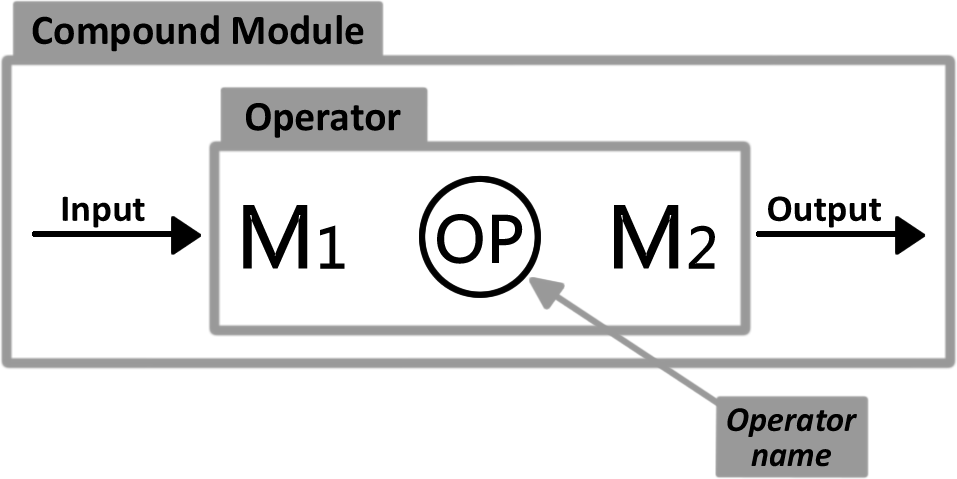
\includegraphics[width=0.5\linewidth]{cm.png}
	\caption[]{A \cm{} made of two modules $M_1$ and $M_2$}
	\label{fig:cm}
\end{figure}

As mentioned before, the \as{} is independent from the \oms{} and \opchs{} used in the solver. It means that one \as{} can be used to construct many different solvers, by implementing it using different modules. %(see below the related concept of \as{} instantiation). 
This is the reason why the \as{} is defined only using {abstract} modules. Formally, we define an \as{} as follows:

\defname{Abstract Solver}{
An \emph{Abstract Solver} $AS$ is a triple $\left(\mathbf{M},\mathcal{L}^m, \mathcal{L}^c\right)$, where: $\mathbf{M}$ is a \cm{} (also called \emph{root \cm{}}), $\mathcal{L}^m$ a list of abstract \oms{} appearing in $\mathcal{M}$, and $\mathcal{L}^c$ a list of \opchs{} appearing in $\mathcal{M}$.}

\Cms{}, and in particular the \textit{root} \cm{}, can be defined also as a context-free grammar as follows:

\begin{definition}\label{def:grammar} A {\bf \cm{}'s grammar} is the set $G_{POSL} = \left(\mathbf{V},\Sigma, \mathbf{S}, \mathbf{R}\right)$, where:
\begin{enumerate}\renewcommand{\labelitemi}{\scriptsize$\blacksquare$}
	\item $\mathbf{V} = \left\{CM, OP\right\}$ is the set of {\it variables},
	\item $\Sigma = \left\{\alpha, \beta, be, [, ], \lbk, \rbk_p, \llparenthesis, \rrparenthesis^m, \rrparenthesis^o, \circled{$\mapsto$},\circled{?},\circlearrowleft, \circled{$\rho$}, \circled{$\vee$}, \circled{$\wedge$}, \circled{M}, \circled{m}, \circled{$\shortdownarrow$}, \circled{$\cup$}, \circled{$\cap$}\right\}$ is the set of {\it terminals},
	\item $\mathbf{S} = \left\{CM\right\}$ is the set of {\it start variables},
	\item and $\mathbf{R} = $
		\begin{align*} 
		CM \produce & \alpha \OR \beta \OR \llparenthesis CM \rrparenthesis^o \OR \llparenthesis CM \rrparenthesis^m \OR \left[OP\right] \OR \lbk OP\rbk_p\\
		OP \produce & CM \circled{$\mapsto$} CM \OR CM \circled{?} CM \OR CM \circled{$\rho$} CM \OR CM \circled{$\vee$} CM \OR CM \circled{$\wedge$} CM  \OR\\
		& CM \circled{M} CM \OR CM \circled{m} CM \OR CM \circled{$\shortdownarrow$} CM \OR CM \circled{$\cup$} CM \OR CM \circled{$\cap$} CM  \OR\\
		& CM \circlearrowleft \text{ be } CM%\left\{CM\right\}		
		\end{align*} is a set of {\it rules}
\end{enumerate} 
%For simplicity, we will use, from now on, the name of \emph{Module} to refer ether to an \module, to an \opch, or to a \cm.
\end{definition}

In the following I explain some of the concepts in Definition~\ref{def:grammar}: 
\begin{itemize}
	\item The variables $CM$ and $OP$ correspond to a \cm{} and an {\it operator}, respectively.
	\item The terminals $\alpha$ and $\beta$ represent a \om{} and a \opch{}, respectively.
	\item The terminal $be$ is a boolean expression.
	\item The terminals $[\text{ } ], \lbk\text{ } \rbk_p$ are symbols for grouping and defining the way the involved \cms{} are executed. Depending on the nature of the operator, this can be either sequentially or in parallel:
	\begin{enumerate}\renewcommand{\labelitemi}{\scriptsize$\blacksquare$}
		\item $\left[\text{OP}\right]$: The involved operator will always executed sequentially.
		\item $\lbk\text{OP}\rbk_p$: The involved operator will be executed in parallel if and only if \emph{OP} supports parallelism. Otherwise, an exception is thrown.
	\end{enumerate}
	\item The terminals $\llparenthesis. \rrparenthesis^m, \llparenthesis.\rrparenthesis^o,$ are operators to send information to other solvers (explained bellow).
	\item All other terminals are \posl{} operators that are detailed later.
\end{itemize}

In the following we define \posl{} operators. In order to group modules, like in Definition~\ref{def:module}(\ref{subdef:seq}) and \ref{def:module}(\ref{subdef:par}), we will use $\left|OP\right|$ as generic grouper. \modified{In order to help the reader to easily understand how to use operators, I use an example of a solver that I build step by step, while presenting the definitions.}

%\begin{example}
%\mybox{Example}
\poslexample{
\posl{} creates solvers based on local search meta-heuristics algorithms. These algorithms have a common structure: \begin{inparaenum}[1.] \item They start by initializing some data structures (e.g., a \emph{tabu list} for \emph{Tabu Search}, a \emph{temperature} for \emph{Simulated Annealing}, etc.). \item An initial configuration $s$ is generated. \item A new configuration $s'$ is selected from the neighborhood $\mathcal{V}\left(s\right)$. \item If $s'$ is a solution for the problem $P$, then the process stops, and $s'$ is returned. If not, the data structures are updated, and $s'$ is accepted or not for the next iteration, depending on a certain criterion. \end{inparaenum}
%An example of such data structure is the penalizing features of local optima in \emph{Guided Local Search} algorithm.

Abstract \oms{} composing local search meta--heuristics are:

\begin{list}{\boxed{Abstract\hspace{4pt}computation\hspace{4pt}module- \arabic{qcounter}~}}{\usecounter{qcounter}} \itemsep0em 
	\item $I$: Generating a configuration $s$
	\item $V$: Defining the neighborhood $\mathcal{V}\left(s\right)$
	\item $S$: Selecting $s' \in \mathcal{V}\left(s\right)$
	\item $A$: Evaluating an acceptance criterion for $s'$
\end{list}
} %\end{example}

The list of modules to be used in the examples have been presented. Now I present \posl{} operators.

\separation

\begin{definition}\label{op:seqexec}
$\circled{$\mapsto$}$ {\bf Sequential Execution Operator.} Let
\begin{enumerate}%\begin{inparaenum}[i)]
	\item $\mathcal{M}_1 : \mathcal{D}_1 \rightarrow \mathcal{I}_1$ and 
	\item $\mathcal{M}_2 : \mathcal{D}_2 \rightarrow \mathcal{I}_2$, 
\end{enumerate}%\end{inparaenum} 
be modules, where $\mathcal{I}_1 \subseteq \mathcal{D}_2$. Then the operation $\left|\mathcal{M}_1\circled{$\mapsto$} \mathcal{M}_2\right|$ defines the \cm{} $\mathcal{M}_{seq}$ as the result of executing $\mathcal{M}_1$ followed by executing $\mathcal{M}_2$:

\[
\mathcal{M}_{seq}:\mathcal{D}_1 \rightarrow \mathcal{I}_2
\]
\end{definition}

This is an example of an operator that does not support the execution of its involved \cms{} in parallel, because the input of the second \cm{} is the output of the first one.

\poslexample{
Coming back to the example, I can use defined abstract \oms{} to create a \cm{} that perform only one iteration of a local search, using the {\bf Sequential Execution} operator. I create a \cm{} to execute sequentially $I$ and $V$ (see Figure~\ref{subfig:ex_seq1}), then I create an other \cm{} to execute sequentially the \cm{} already created and $S$ (see Figure~\ref{subfig:ex_seq2}), and finally this \cm{} and the \om{} $A$ are executed sequentially (see Figure~\ref{subfig:ex_seq3}). The \cm{} presented in Figure~\ref{subfig:ex_seq3} can be coded as follows:
$$\left[\left[\left[I\poslop{\mapsto}V\right]\poslop{\mapsto}S\right]\poslop{\mapsto}A\right]$$
In the figure, each rectangle is a \cm.
}

\begin{figure}[h]
	\centering
	\subfloat[][]{
		\label{subfig:ex_seq1}
		
\includegraphics[width=0.2\linewidth]{seq_1.png}
	}\hspace{0.05\linewidth}
	\subfloat[][]{%
		\label{subfig:ex_seq2}
		
\includegraphics[width=0.3\linewidth]{seq_2.png}
	}\\
	\subfloat[][]{%
		\label{subfig:ex_seq3}
		
\includegraphics[width=0.4\linewidth]{seq_3.png}
	}
	\caption[]{Using {\bf sequential execution} operator}
	\label{fig:seq_example}
\end{figure}

\separation

The following operator is very useful to execute modules sequentially creating bifurcations, subject to some boolean condition:

\begin{definition}\label{op:conditional}
$\circled{?}$ {\bf Conditional Execution Operator} Let
\begin{enumerate}%\begin{inparaenum}[i)]
	\item $\mathcal{M}_1 : \mathcal{D}_1 \rightarrow \mathcal{I}_1$ and  
	\item $\mathcal{M}_2 : \mathcal{D}_2 \rightarrow \mathcal{I}_2$,
\end{enumerate}%\end{inparaenum} 
be modules, where $\mathcal{D}_1 \cap \mathcal{D}_2 \neq \emptyset$. %and $\mathcal{I}_1 \subset \mathcal{I}_2$. 
Then the operation $\left|\mathcal{M}_1\circled{?}_{<cond>}\mathcal{M}_2\right|$ defines the \cm{} $\mathcal{M}_{cond}$ as result of the sequential execution of $\mathcal{M}_1$ if $<cond>$ is {\bf true} or $\mathcal{M}_2$, otherwise:

\[
\mathcal{M}_{cond}:\mathcal{D}_1\cap\mathcal{D}_2 \rightarrow \mathcal{I}_1 \cup \mathcal{I}_2 
\]
\end{definition}

\poslexample{
This operator can be used in the example if I want to execute two different {\it selection} \oms{} ($S_1$ and $S_2$) depending on certain criterion (see Figure~\ref{fig:cond_example}):
$$\left[\left[\left[I\poslop{\mapsto}V\right]\poslop{\mapsto}\left[S_1\poslop{?}S_2\right]\right]\poslop{\mapsto}A\right]$$
In examples I remove the clause $<cond>$ for simplification.
}

\begin{figure}[h]
	\centering	
	
\includegraphics[width=0.5\linewidth]{cond.png}
	\caption{Using {\bf conditional execution} operator}\label{fig:cond_example}
\end{figure}

\separation

We can execute modules sequentially creating also cycles.

\begin{definition}\label{op:cyclic}
$\circlearrowleft$ {\bf Operator Cyclic Execution Operator} Let $\mathcal{M} : \mathcal{D} \rightarrow \mathcal{I}$ be a module, where $\mathcal{I} \subseteq \mathcal{D}$. Then, the operation $\left|\circlearrowleft_{<cond>}\mathcal{M}\right|$ defines the \cm{} $\mathcal{M}_{cyc}$ repeating sequentially the execution of $\mathcal{M}$ while $<cond>$ remains {\bf true}:

\[
\mathcal{M}_{cyc}:\mathcal{D} \rightarrow \mathcal{I} 
\]
\end{definition}

\poslexample{
Using this operator I can model a local search algorithm, by executing the {\it abstract} \om{} $I$ and then the other \oms{} ($V$, $S$ and $A$) cyclically, until finding a solution (i.e, a configuration with cost equals to zero) (see Figure~\ref{fig:cyc_example}):
$$\left[I\poslop{\mapsto}\left[\circlearrowleft\left[\left[V\poslop{\mapsto}S\right]\poslop{\mapsto}A\right]\right]\right]$$
In the examples, I remove the clause $<cond>$ for simplification. 
}

\begin{figure}[h]
	\centering	
	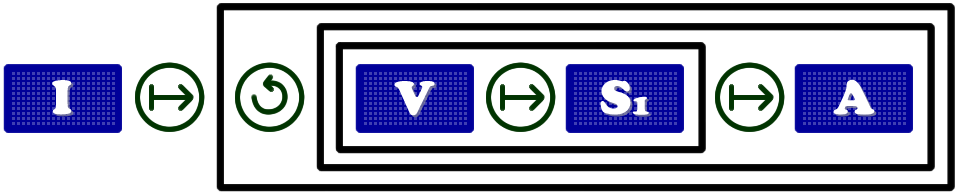
\includegraphics[width=0.5\linewidth]{cyc.png}
	\caption{Using {\bf cyclic execution} operator}\label{fig:cyc_example}
\end{figure}

\separation

\begin{definition}\label{op:rho}
{\bf (Operator Random Choice)} Let
\begin{enumerate}%\begin{inparaenum}[i)]
	\item $\mathcal{M}_1 : \mathcal{D}_1 \rightarrow \mathcal{I}_1$ and  
	\item $\mathcal{M}_2 : \mathcal{D}_2 \rightarrow \mathcal{I}_2$,
\end{enumerate}%\end{inparaenum} 
be modules, where $\mathcal{D}_1 \subset \mathcal{D}_2$, % and $\mathcal{I}_1 \subset \mathcal{I}_2$, 
and a real value $\rho \in (0,1)$. Then the operation $\left|M_1\circled{$\rho$}\mathcal{M}_2\right|$ defines the \cm{} $\mathcal{M}_{rho}$ executing $\mathcal{M}_1$ with probability $\rho$, or executing $\mathcal{M}_2$ with probability $(1-\rho)$:

\[
\mathcal{M}_{rho}:\mathcal{D}_1\cap\mathcal{D}_2 \rightarrow \mathcal{I}_1 \cup \mathcal{I}_2 
\]
\end{definition}

\poslexample{
In the example I can create a \cm{} to execute two {\it abstract} \oms{} $A_1$ and $A_2$ following certain probability $\rho$ using the {\bf random choice} operator as follows (see Figure~\ref{fig:rho_example}):
$$\left[I\poslop{\mapsto}\left[\circlearrowleft\left[\left[V\poslop{\mapsto}S\right]\poslop{\mapsto}\left[A_1\poslop{\rho}A_2\right]\right]\right]\right]$$
}

\begin{figure}[h]
	\centering	
	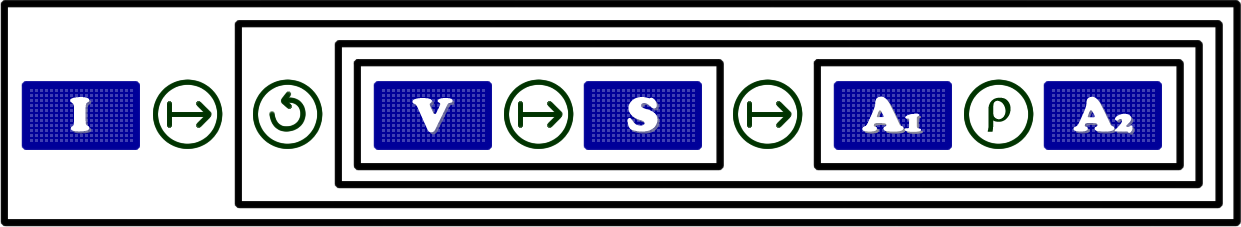
\includegraphics[width=0.6\linewidth]{rho.png}
	\caption{Using {\bf random choice} operator}\label{fig:rho_example}
\end{figure}

\separation

The following operator is very useful if the user needs to use a \opch{} inside an \as{}. As explained before, if a \opch{} does not receive any information from another solver, it returns {\it NULL}. This may cause the undesired termination of the solver if this case is not considered correctly. Next, I introduce the operator \textbf{Operator Not {\it NULL} Execution} and illustrate how to use it in practice with an example.

\begin{definition}\label{op:or}
{\bf (Operator Not {\it NULL} Execution)} Let
\begin{enumerate}%\begin{inparaenum}[i)]
	\item $\mathcal{M}_1 : \mathcal{D}_1 \rightarrow \mathcal{I}_1$ and  
	\item $\mathcal{M}_2 : \mathcal{D}_2 \rightarrow \mathcal{I}_2$,
\end{enumerate}%\end{inparaenum} 
be modules, where $\mathcal{D}_1 \subseteq \mathcal{D}_2$. % and $\mathcal{I}_1 \subset \mathcal{I}_2$. 
Then, the operation $\left|\mathcal{M}_1\circled{$\vee$}\mathcal{M}_2\right|$ defines the \cm{} $\mathcal{M}_{non}$ that executes $\mathcal{M}_1$ and returns its output if it is not {\it NULL}, or executes $\mathcal{M}_2$ and returns its output otherwise:

\[
\mathcal{M}_{non}:\mathcal{D}_1\cap\mathcal{D}_2 \rightarrow \mathcal{I}_1 \cup \mathcal{I}_2 
\]
\end{definition}

\poslexample{Let us make consider a slightly more complex example: When applying the acceptance criterion, suppose that we want to receive a configuration from other solver to combine the \om{} $A$ with a \opch:

\begin{list}{\boxed{Communication\hspace{4pt}module- \arabic{qcounter}:~}}{\usecounter{qcounter}} \itemsep0em
	\item $C.M.$: Receiving a configuration.\label{struct:opch}
\end{list}

Figure~\ref{fig:2difBeh} shows how to combine a \opch{} with the \om{} $A$ through the operator $\circled{$\vee$}$. Here, the \om{} $A$ will be executed as long as the \opch{} remains \textit{NULL}, i.e., there is no information coming from outside. This behavior is represented in Figure~\ref{subfig:beh1} by the orange lines. If some data has been received through the \opch, the later is executed instead of the module $A$, represented in Figure~\ref{subfig:beh2} by blue lines. 
The code can be written as follows:
$$\left[I\poslop{\mapsto}\left[\circlearrowleft\left[\left[V\poslop{\mapsto}S\right]\poslop{\mapsto}\left[A\poslop{\vee}C.M.\right]\right]\right]\right]$$
}

\begin{figure}[h]
\centering
\subfloat[][The solver executes the computation module {\bf A} if no information is received through the connection module]{
	\label{subfig:beh1}
	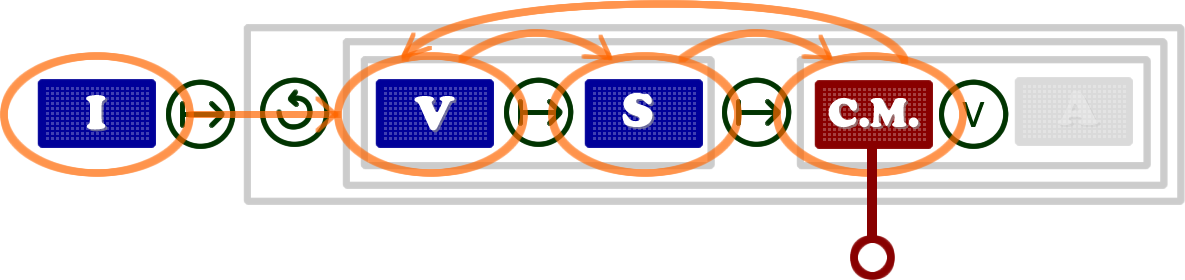
\includegraphics[width=0.6\linewidth]{muta1_v4.png}
}\\
%\hspace{0.05\textwidth}%
\subfloat[][The solver uses the information coming from an external solver]{%
	\label{subfig:beh2}
	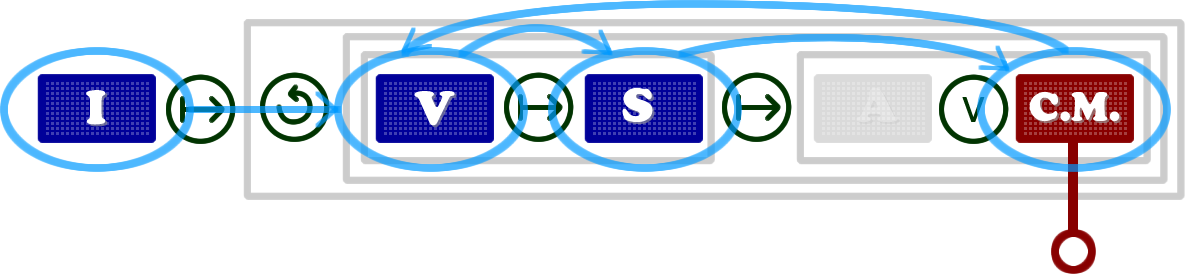
\includegraphics[width=0.6\linewidth]{muta2_v4.png}
}
\caption[]{Two different behaviors within the same solver}
\label{fig:2difBeh}
\end{figure}

This is {\it short-circuit} operator. It means that if the first argument (module) does not return {\it NULL}, the second will not be executed. \posl{} provides another operator with the same functionality but not {\it short-circuit}:

\begin{definition}\label{op:and}
{\bf (Operator {\it BOTH} Execution)} Let 
\begin{enumerate}%\begin{inparaenum}[i)]
	\item $\mathcal{M}_1 : \mathcal{D}_1 \rightarrow \mathcal{I}_1$ and  
	\item $\mathcal{M}_2 : \mathcal{D}_2 \rightarrow \mathcal{I}_2$,
\end{enumerate}%\end{inparaenum} 
be modules, where $\mathcal{D}_1 \subseteq \mathcal{D}_2$. % and $\mathcal{I}_1 \subset \mathcal{I}_2$. 
Then the operation $\left|\mathcal{M}_1\circled{$\wedge$}\mathcal{M}_2\right|$ defines the \cm{} $\mathcal{M}_{both}$ that executes both $\mathcal{M}_1$ and $\mathcal{M}_2$, then returns the output of $\mathcal{M}_1$ if it is not {\it NULL}, or the output of $\mathcal{M}_2$ otherwise:

\[
\mathcal{M}_{both}:\mathcal{D}_1\cap\mathcal{D}_2 \rightarrow \mathcal{I}_1 \cup \mathcal{I}_2 
\]
\end{definition}

In the following definitions, the concepts of {\it cooperative parallelism} and {\it competitive parallelism} are implicitly included. We say that cooperative parallelism exists when two or more processes are running separately, they are independent, and the general result will be some combination of the results of all the involved processes (e.g. Definitions~\ref{op:min} and~\ref{op:max}). \modified{On the other hand, competitive parallelism arise when the general result is the result of the process ending first (e.g. Definition~\ref{op:race}).}

\begin{definition}\label{op:min}
{\bf (Operator Minimum)} Let
\begin{enumerate}%\begin{inparaenum}[i)]
	\item $\mathcal{M}_1 : \mathcal{D}_1 \rightarrow \mathcal{I}_1$ and  
	\item $\mathcal{M}_2 : \mathcal{D}_2 \rightarrow \mathcal{I}_2$,
\end{enumerate}%\end{inparaenum} 
be modules, where $\mathcal{D}_1 \subseteq \mathcal{D}_2$. %and $\mathcal{I}_1 \subset \mathcal{I}_2$. 
Let also $o_1$ and $o_2$ be the outputs of $\mathcal{M}_1$ and $\mathcal{M}_2$, respectively. Assume that there exists some order criteria between them. Then the operation $\left|\mathcal{M}_1\circled{m}\mathcal{M}_2\right|$ defines the \cm{} $\mathcal{M}_{min}$ that executes $\mathcal{M}_1$ and returns $\min\left\{o_1,o_2\right\}$:

\[
\mathcal{M}_{min}:\mathcal{D}_1\cap\mathcal{D}_2 \rightarrow \mathcal{I}_1 \cup \mathcal{I}_2 
\]
\end{definition}

Similarly we define the operator \textbf{Maximum}:

\begin{definition}\label{op:max}
{\bf (Operator Maximum)} Let
\begin{enumerate}%\begin{inparaenum}[i)]
	\item $\mathcal{M}_1 : \mathcal{D}_1 \rightarrow \mathcal{I}_1$ and  
	\item $\mathcal{M}_2 : \mathcal{D}_2 \rightarrow \mathcal{I}_2$,
\end{enumerate}%\end{inparaenum} 
be modules, where $\mathcal{D}_1 \subseteq \mathcal{D}_2$. %and $\mathcal{I}_1 \subset \mathcal{I}_2$. 
Let also $o_1$ and $o_2$ be the outputs of $\mathcal{M}_1$ and $\mathcal{M}_2$, respectively. Assume that there exists some order criteria between them. Then the operation $\left|\mathcal{M}_1\circled{M}\mathcal{M}_2\right|$ defines the \cm{} $\mathcal{M}_{max}$ that executes $\mathcal{M}_1$ and returns $\max\left\{o_1,o_2\right\}$:

\[
\mathcal{M}_{max}:\mathcal{D}_1\cap\mathcal{D}_2 \rightarrow \mathcal{I}_1 \cup \mathcal{I}_2 
\]
\end{definition}

\poslexample{Comming back to the previews example, the {\bf minimum operator} can be applied to obtain a more interesting behavior in the solver: When applying the acceptance criteria, suppose that we want to receive a configuration from other solver, to compare it with ours and select the one with the lowest cost. We can do that by applying the operator~$\circled{m}$ to combine the \om{} $A$ with a \opch{} $C.M.$ (see Figure\ref{fig:min_example}):
$$\left[I\poslop{\mapsto}\left[\circlearrowleft\left[\left[V\poslop{\mapsto}S\right]\poslop{\mapsto}\lbk A\poslop{m}C.M.\rbk_p\right]\right]\right]$$
Notice that in this example, I can use the grouper $\lbk .\rbk_p$ since the {\bf minimum operator} supports parallelism.}

\begin{figure}[h]
	\centering	
	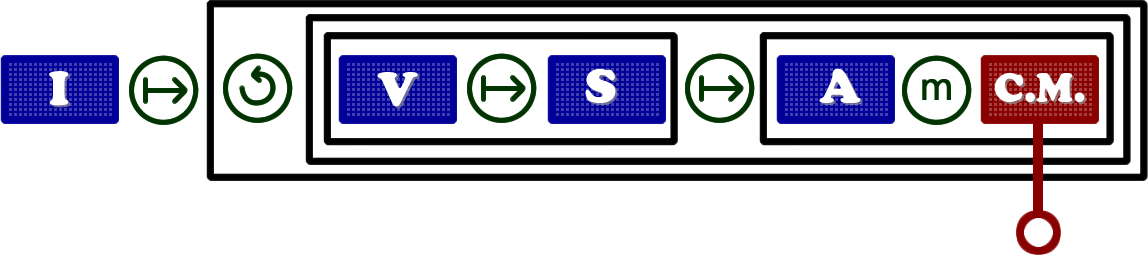
\includegraphics[width=0.6\linewidth]{min.png}
	\caption{Using {\bf minimum} operator}\label{fig:min_example}
\end{figure}

\begin{definition}\label{op:race}
{\bf (Operator Race)} Let 
\begin{enumerate}%\begin{inparaenum}[i)]
	\item $\mathcal{M}_1 : \mathcal{D}_1 \rightarrow \mathcal{I}_1$ and  
	\item $\mathcal{M}_2 : \mathcal{D}_2 \rightarrow \mathcal{I}_2$,
\end{enumerate}%\end{inparaenum} 
be modules, where $\mathcal{D}_1 \subseteq \mathcal{D}_2$ and $\mathcal{I}_1 \subset \mathcal{I}_2$. Then the operation $\left|\mathcal{M}_1\circled{$\shortdownarrow$}\mathcal{M}_2\right|$ defines the \cm{} $\mathcal{M}_{race}$ that executes both modules $\mathcal{M}_1$ and $\mathcal{M}_2$, and returns the output of the module ending first:

\[
\mathcal{M}_{race}:\mathcal{D}_1\cap\mathcal{D}_2 \rightarrow \mathcal{I}_1 \cup \mathcal{I}_2 
\]
\end{definition}

\poslexample{Sometimes nighborhood functions are slow depending on the configuration. In that case two neighborhood \oms{} can be executed and take into account the output of the module ending first (see Figure\ref{fig:race_example}):
$$\left[I\poslop{\mapsto}\left[\circlearrowleft\left[\left[\lbk V_1\poslop{\shortdownarrow}V_2\rbk_p\poslop{\mapsto}S\right]\poslop{\mapsto}\lbk A\poslop{m}C.M.\rbk_p\right]\right]\right]$$}

\begin{figure}[h]
	\centering	
	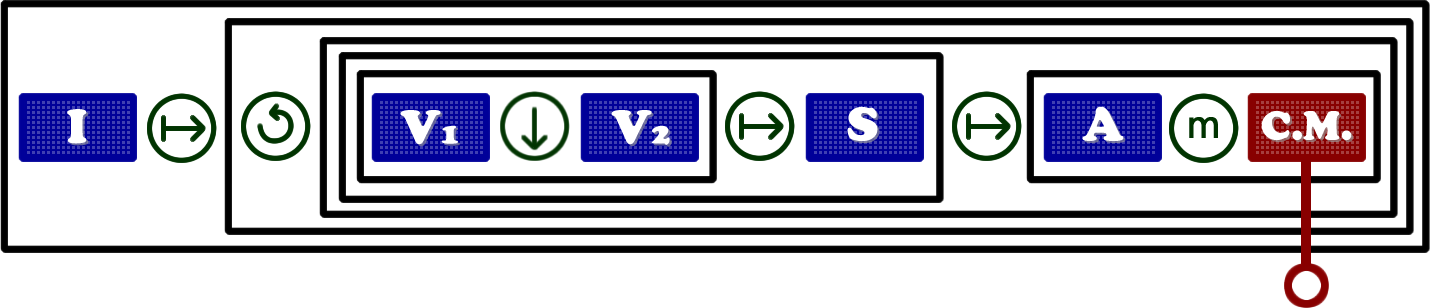
\includegraphics[width=0.7\linewidth]{race.png}
	\caption{Using {\bf race} operator}\label{fig:race_example}
\end{figure}

Some others operators can be useful when dealing with {\it sets}.

\begin{definition}\label{op:union}
{\bf (Operator Union)} Let 
\begin{enumerate}%\begin{inparaenum}[i)]
	\item $\mathcal{M}_1 : \mathcal{D}_1 \rightarrow \mathcal{I}_1$ and  
	\item $\mathcal{M}_2 : \mathcal{D}_2 \rightarrow \mathcal{I}_2$,
\end{enumerate}%\end{inparaenum} 
be modules, where $\mathcal{D}_1 \subseteq \mathcal{D}_2$. %and $\mathcal{I}_1 \subset \mathcal{I}_2$. 
Let also $V_1$ and $V_2$ be the outputs of $\mathcal{M}_1$ and $\mathcal{M}_2$, respectively. Then the operation $\left|\mathcal{M}_1\circled{$\cup$}\mathcal{M}_2\right|$ defines the \cm{} $\mathcal{M}_{\cup}$ that executes both modules $\mathcal{M}_1$ and $\mathcal{M}_2$, and returns $V_1\cup V_2$:

\[
\mathcal{M}_{\cup}:\mathcal{D}_1\cap\mathcal{D}_2 \rightarrow \mathcal{I}_1 \cup \mathcal{I}_2
\]
\end{definition}

Similarly we define the operators \textbf{Intersection} and \textbf{Subtraction}:

\begin{definition}\label{op:intersec}
{\bf (Operator Intersection)} Let 
\begin{enumerate}%\begin{inparaenum}[i)]
	\item $\mathcal{M}_1 : \mathcal{D}_1 \rightarrow \mathcal{I}_1$ and  
	\item $\mathcal{M}_2 : \mathcal{D}_2 \rightarrow \mathcal{I}_2$,
\end{enumerate}%\end{inparaenum} 
be modules, where $\mathcal{D}_1 \subseteq \mathcal{D}_2$. % and $\mathcal{I}_1 \subset \mathcal{I}_2$. 
Let also $V_1$ and $V_2$ be the outputs of $\mathcal{M}_1$ and $\mathcal{M}_2$, respectively. Then the operation $\left|\mathcal{M}_1\circled{$\cap$}\mathcal{M}_2\right|$ defines the \cm{} $\mathcal{M}_{\cap}$ that executes both modules $\mathcal{M}_1$ and $\mathcal{M}_2$, and returns $V_1\cap V_2$:

\[
\mathcal{M}_{\cap}:\mathcal{D}_1\cap\mathcal{D}_2 \rightarrow \mathcal{I}_1 \cup \mathcal{I}_2
\]
\end{definition}

\begin{definition}\label{op:subst}
{\bf (Operator Subtraction)} Let 
\begin{enumerate}%\begin{inparaenum}[i)]
	\item $\mathcal{M}_1 : \mathcal{D}_1 \rightarrow \mathcal{I}_1$ and  
	\item $\mathcal{M}_2 : \mathcal{D}_2 \rightarrow \mathcal{I}_2$,
\end{enumerate}%\end{inparaenum} 
be modules, where $\mathcal{D}_1 \subseteq \mathcal{D}_2$. % and $\mathcal{I}_1 \subset \mathcal{I}_2$. 
Let also $V_1$ and $V_2$ be the outputs of $\mathcal{M}_1$ and $\mathcal{M}_2$, respectively. Then the operation $\left|\mathcal{M}_1\circled{-}\mathcal{M}_2\right|$ defines the \cm{} $\mathcal{M}_{-}$ that executes both modules $\mathcal{M}_1$ and $\mathcal{M}_2$, and returns $V_1 - V_2$:

\[
\mathcal{M}_{-}:\mathcal{D}_1\cap\mathcal{D}_2 \rightarrow \mathcal{I}_1 \cup \mathcal{I}_2
\]
\end{definition}

Now, I define the operators which allows to send information to other solvers. Two types of information can be sent: 
\begin{inparaenum}[i)]
	\item the output of the \om{} and send its output, or 
	\item the \om{} itself.
\end{inparaenum}. This utility is very useful in terms of sharing behaviors between solvers.

\begin{definition}\label{op:osend}
{\bf (Sending Data Operator)} Let $\mathcal{M} : \mathcal{D} \rightarrow \mathcal{I}$ be a module. Then the operation $\left|\llparenthesis \mathcal{M}\rrparenthesis^{o}\right|$ defines the \cm{} $\mathcal{M}_{sendD}$ that executes the module $\mathcal{M}$ and sends its output outside:

\[
\mathcal{M}_{sendD}:\mathcal{D} \rightarrow \mathcal{I}
\]
\end{definition}

Similarly we define the operator \textbf{Send Module}:

\begin{definition}\label{op:msend}
{\bf (Sending Module Operator)} Let $\mathcal{M} : \mathcal{D} \rightarrow \mathcal{I}$ be a module. Then the operation $\left|\llparenthesis \mathcal{M}\rrparenthesis^{m}\right|$ defines the \cm{} $\mathcal{M}_{sendM}$ that executes the module $\mathcal{M}$, then returns its output and sends the module itself outside:

\[
\mathcal{M}_{sendM}:\mathcal{D} \rightarrow \mathcal{I}
\]
\end{definition}

\poslexample{In the following example, I use one of the \cms{} already presented in the previews examples, using a \opch{} to receive a configuration (see Figure~\ref{subfig:receiver_example}):  
$$\left[I\poslop{\mapsto}\left[\circlearrowleft\left[\left[V\poslop{\mapsto}S\right]\poslop{\mapsto}\lbk A\poslop{m}C.M.\rbk_p\right]\right]\right]$$

I also build another, as its complement: sending the accepted configuration to outside, using the {\bf sending data operator} (see Figure\ref{subfig:sender_example}):
$$\left[I\poslop{\mapsto}\left[\circlearrowleft\left[\left[V\poslop{\mapsto}S\right]\poslop{\mapsto}\llparenthesis A\rrparenthesis^{o}\right]\right]\right]$$

In the Section~\ref{sec:4thstage} I explain how to connect solvers to each other.
}

\begin{figure}[h]
\centering
\subfloat[][]{
	\label{subfig:receiver_example}
	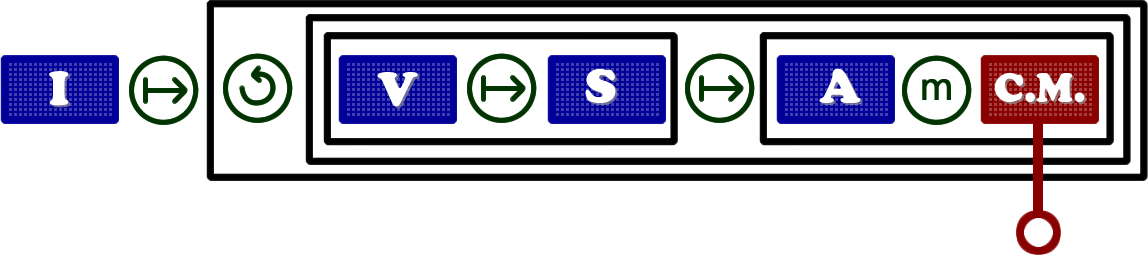
\includegraphics[width=0.6\linewidth]{min.png}
}\\
\subfloat[][]{%
	\label{subfig:sender_example}
	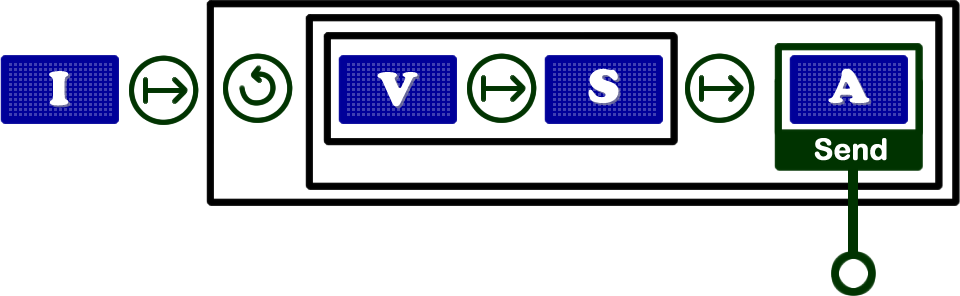
\includegraphics[width=0.6\linewidth]{send.png}
}
\caption[]{Sender and receiver behaviors}
\label{fig:send_recv}
\end{figure}

Once all desired abstract modules are linked together with operators, we obtain the {\it root} \cm{}, an important part of an \as. To implement a concrete solver from an \as, one must instantiate each abstract module with a concrete one respecting the required signature. From the same \as, one can implement many different concrete solvers simply by instantiating abstract modules with different concrete modules.

An \as{} is defined as follows: after declaring the \mbox{\tet{\bf abstract solver}}'s name, the first line defines the list of abstract \oms, the second one the list of abstract \opchs, then the algorithm of the solver is defined as the solver's body (the root \cm), between \mbox{\tet{\bf begin}} and \mbox{\tet{\bf end}}.

An \as{} can be declared through the  simple regular expression:

\begin{center}
\tet{\bf abstract solver} {\it name} \tet{\bf computation}: $L^m$ (\tet{\bf communication}: $L^c$)? \tet{\bf begin} $\mathcal{M}$ \tet{\bf end}
\end{center}

where:
\begin{itemize}
\item {\it name} is the identifier of the \as{}, 
\item $L^m$ is the list of abstract \oms{},
\item $L^c$ is the list of abstract \opchs{}, and
\item $\mathcal{M}$ is the root \cm.
\end{itemize}

For instance, Algorithm~\ref{algo:as_example} illustrates the abstract solver corresponding to Figure~\ref{subfig:as}.

\begin{algorithm}[H]
\dontprintsemicolon
\SetNoline
\SetKwProg{myproc}{}{}{}
\myproc{\tet{\bf abstract solver} as\_01\;
\tet{\bf computation} : $I, V, S, A$ \; 
\tet{\bf connection}: $C.M.$}{
	\Begin{
		%\While{$($\Iter $< K_1)$}
		%{
			$I$ \sec \; %\circled{$\mapsto$}$\;
			\While{$($\Iter \% $K_1)$}{
				$\left[V\poslop{\mapsto}S\poslop{\mapsto}\left[C.M.\poslop{m} \llparenthesis A\rrparenthesis^o\right]\right]$\;
			}
		%}
	}
}
\caption{\posl{} pseudo-code for the \as{} presented in Figure~\ref{subfig:as}}\label{algo:as_example}
\end{algorithm}	